% !TEX root = diss.tex

\chapter{Introduction}

Hydrogen atom transfer (HAT) reactions involve chemical species with an odd
number of electrons, or free radicals. These fundamental chemical
transformations have been studied extensively for over a
century.\cite{Kochi1973,Parsons2000} All HAT reactions involve the transfer of
at least one hydrogen atom (\ch{H^.}), although there exist various mechanisms
by which this can occur. Free radicals and HAT reactions play an important role
in many chemical and biological processes.\cite{Halliwell2015}

\section{Processes involving hydrogen transfer reactions}

\subsection{Hydrogen atom transfer reactions in biological processes}

In biology, oxygen centred radicals are referred to as reactive oxygen species
(ROSs). Nearly all ROSs derive from the metabolic processes involving molecular
oxygen, \ch{O2}.\cite{Barnham2004} At conditions relevant to biology, organic
matter exists in the singlet ground state while \ch{O2} exists in a triplet
ground state: the quantum mechanical selection rule prohibits electronic
interactions. As a result, evolution has driven organisms to develop techniques
to overcome this. Most commonly, enzymes containing transition metals are used
to activate \ch{O2}, producing reactive radical intermediates or products,
i.e. ROSs. ROSs play an important role in normal biological functions, however
an ``imbalance'' may lead to the oxidation of important biomaterials, or
oxidative stress.\cite{Halliwell2015} In humans, oxidative stress has been
linked to many degenerative disease states such as Alzheimer's
disease,\cite{Barnham2004,Valko2007} Parkinson's disease,\cite{Hwang2013}
ageing, and cancer.\cite{Halliwell2007}

It is widely accepted that the vast majority of ROSs originate from reactions of
\ch{O2} with the redox-active metals copper and iron.\cite{Halliwell2015} A
common example is the Haber-Weiss reaction, the second step in the Fenton cycle
(Equations~\ref{eq:fen1}~--~\ref{eq:fennet}):

\begin{align}
\centering
\ch{Fe^{3+} + ^.O2^- &-> Fe^{2+} + O2} \label{eq:fen1}\\
\ch{Fe^{2+} + H2O2 &-> Fe^{3+} + OH^- + ^.OH} \label{eq:fen2}\\
\cline{1-2}
\ch{^.O2^- + H2O2 &-> ^.OH + OH^- + O2}\label{eq:fennet}
\end{align}

\noindent It is the production of the highly reactive hydroxyl radical
(\ch{^.OH}) which is responsible for the initiation of the majority of oxidative
stress through the abstraction of a hydrogen atom. Given its very short \emph{in
  vivo} half-life of about $10^{-9}$ s, \ch{^.OH} reacts with practically all
biomaterials.\cite{Sies1993}

DNA and RNA are susceptible to radical damage,\cite{Halliwell2015,Valko2007} and
reactions of \ch{^.OH} with DNA molecules have been studied in some
detail. Damage can occur to both the pyrimidine and purine bases, as well as the
deoxyribose backbone, with over 20 DNA lesions having been
identified.\cite{Dizdaroglu1992,Cooke2003} The most commonly studied product is
8-hydroxyguanine (or the tautomer 8-oxo-2$'$-deoxyguanosine), which is the
result of the oxidation of the guanine nitrogenous base. This particular
oxidation can result in mismatched base pairing of guanosine with adenine
(rather than cytosine), contrary to the Watson-Crick model, leading to possible
substitutions in the genome.\cite{Cheng1992} It is important to realise that
although there are enzymes which actively repair DNA and remove
lesions,\cite{Friedberg2005} oxidation represents the permanent modification of
genetic material which is the first step in mutagenesis, carcinogenesis, and
ageing.

Polyunsaturated fatty acids are extremely sensitive to oxidation. Specifically,
the autoxidation of polyunsaturated fatty acids and esters occurs rapidly, and
has been intensely
investigated.\cite{Marnett2000,Sevanian2000,Pratt2003,Spiteller2007,Ayala2014}
This radical chain reaction is initiated by reactions of lipids with \ch{^.OH}
forming a pentadienyl radical. Oxygen adds rapidly (although reversibly) to the
intermediate carbon radical,\cite{Pratt2003} giving a lipid peroxyl radical
(\ch{LOO^.}). Once formed, \ch{LOO^.} can propagate to form further carbon
centred radicals, terminate through the reaction with another \ch{LOO^.}, or can
rearrange through a cyclisation reaction to form an endoperoxide. The
endoperoxide product reacts further to produce mainly aldehydes, and most
predominantly malondialdehyde (MDA).\cite{Valko2007} MDA is highly reactive and
has been shown to be either mutagenic or carcinogenic in mammalian and bacterial
models.\cite{Marnett2000}

Our work is primarily concerned with models for proteins. The oxidation of
protein by ROSs occurs through a radical chain mechanism which has been studied
in detail.\cite{Berlett1997} Through experiments in which proteins were exposed
to ionising radiation, it was demonstrated that protein oxidation is initiated
through hydrogen atom transfer (HAT) reactions with \ch{^.OH}. The propagation
often occurs through radical-mediated oxidation, as illustrated in
\ref{fig:proteinoxidation}.

\begin{scheme}[h!]
  \begin{center}
  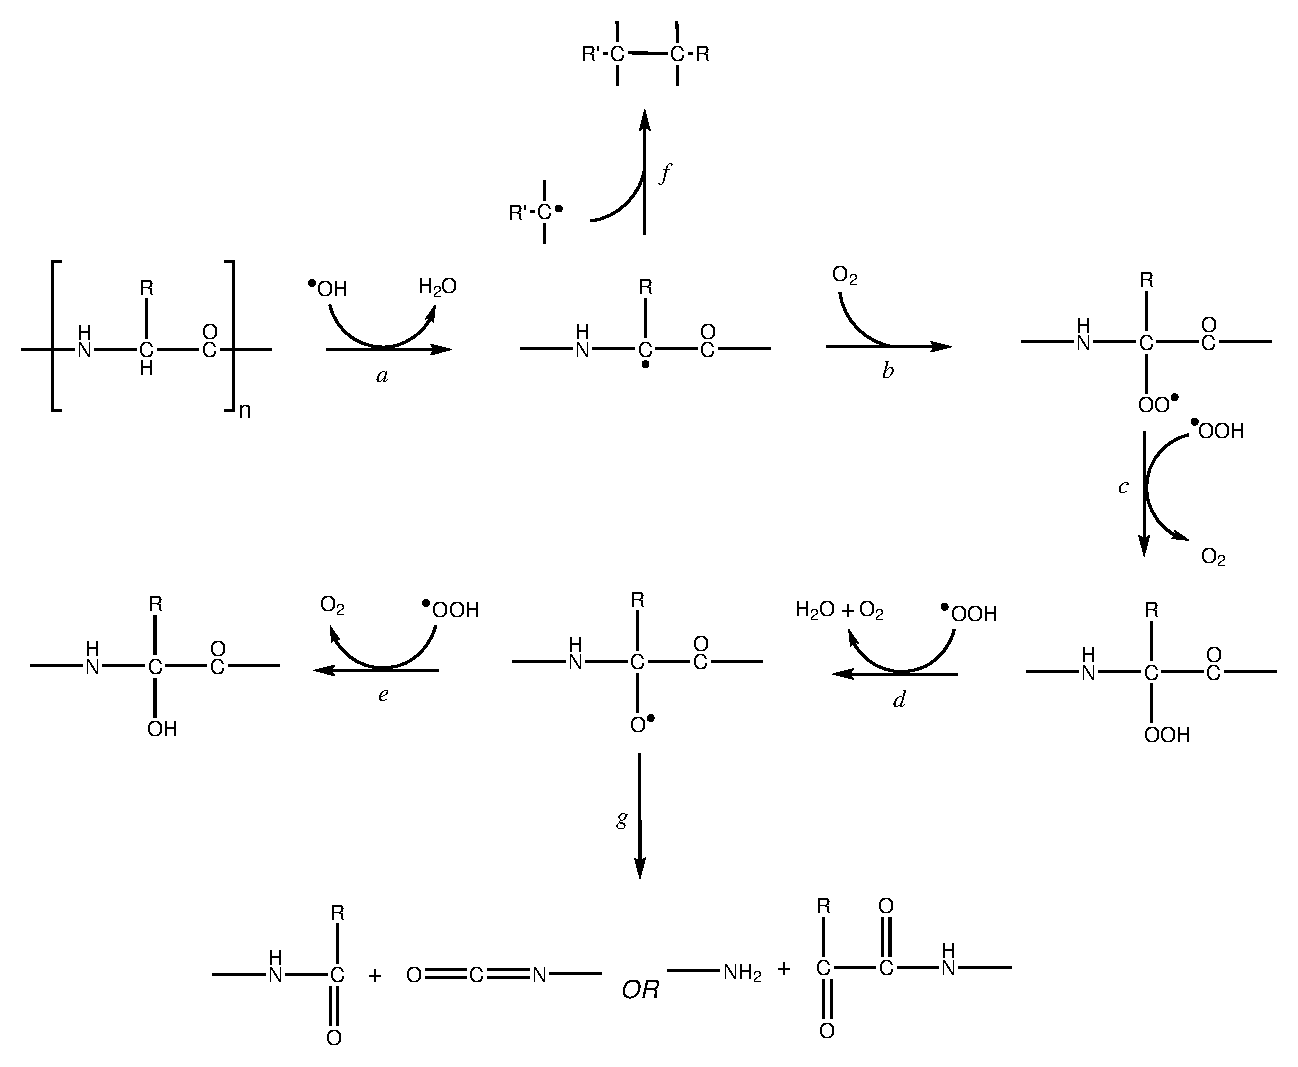
\includegraphics[width=\textwidth]{figures/proteinoxidation.eps}
  \caption[Common reactions involved in radical-mediated oxidation of
  proteins]{Common reaction involved in radical-meditated oxidation of
    proteins. The reactions are as follows: \emph{a} initiation or radical chain
    through abstraction by the hydroxyl radical, \emph{b} radical addition of
    molecular oxygen, \emph{c} HAT with an incipient peroxyl radical, \emph{d}
    additional reaction with an incipient peroxyl radical producing water and
    oxygen, \emph{e} termination by HAT with an incipient peroxyl radical,
    \emph{f} possible cross-linking mechanism of two carbon centred radicals
    \emph{g} possible fragmentation pathways of an oxygen centred radical
    intermediate. Figure adapted from Reference \protect\citenum{Berlett1997}.}
\label{fig:proteinoxidation}
  \end{center}
\end{scheme}

Initial abstraction occurs primarily at the $\alpha$-carbon position (Reaction
$a$), although the side-chains are also susceptible to oxidation.  Those
side-chains containing sulfur,\cite{Stadtman2004} as well as tyrosine (which has
a fairly weak phenolic O-H bond of about 89 \kcalmol),\cite{Mulder2005} are
particularly susceptible to oxidation. The course of propagation through radical
mediated protein oxidation is determined by the availability of either singlet
oxygen (\ch{^1O2}), or superoxide (\ch{O2^{.-}}) (or the protonated form,
hydroxyl radical (\ch{^.OOH})). Reactions that proceed with singlet oxygen are
shown in $b$-$e$. The radical chain reaction can be terminated through two
mechanisms, protein-protein cross-linking (Reaction $f$) or protein
fragmentation (Reaction $g$). These processes lead to the accumulation of
oxidised proteins which is associated with many degenerative
diseases.\cite{Halliwell2006}


\subsection{Hydrogen atom transfer reaction in chemical processes}

Given the importance of HAT reaction in biological systems, it seems obvious for
chemists to develop means in which this tool can be used as well. Given the
highly reactive nature of free radicals, this has certainly been a challenge.
However, there exists multiple examples of utilising HAT reactions in important
energy conversion processes,\cite{Hammes-Schiffer2012} as well as in chemical
synthesis.\cite{Balcells2016,Miller2016}

In organic synthesis, the replacement of specific C-H bonds (C-H bond
functionalisation) has long been of interest. One such way to achieve this is
through radical reactions.\cite{Godula2006} Intramolecular radical reactions
were first utilised in the late 1800s when Hofmann showed that homolysis of
bromamines and chloramines lead to functionalisation of $\delta$-methylene or
methyl groups.\jnote{citation needed, see \citet{Godula2006}} Now called the
Hofmann-L{\"o}fler-Freytag reaction, this reaction is used to form cyclic
amines, and proceeds through an intramolecular HAT, as shown in
\ref{fig:hofmann}. The reaction is initiated by the cleavage of a
nitrogen-halogen bond, either by radiation or a radical initiator. Next is a key
intramolecular HAT reaction that proceeds through a six-membered cyclic
transition state which can adopt an unstrained chair conformation.  Another
related reaction is the Barton reaction\cite{Barton1960} which involves
photo-initiated homolytic cleavage of a nitrite (RO-NO) bond, followed by
$\delta$-hydrogen abstraction, and radical coupling to form a $\delta$-nitroso
alcohol. The Hofmann-L{\"o}fler-Freytag reaction served as a proof of concept
that HAT could be useful in synthetic chemistry.

\begin{scheme}[htb]
  \begin{center}
  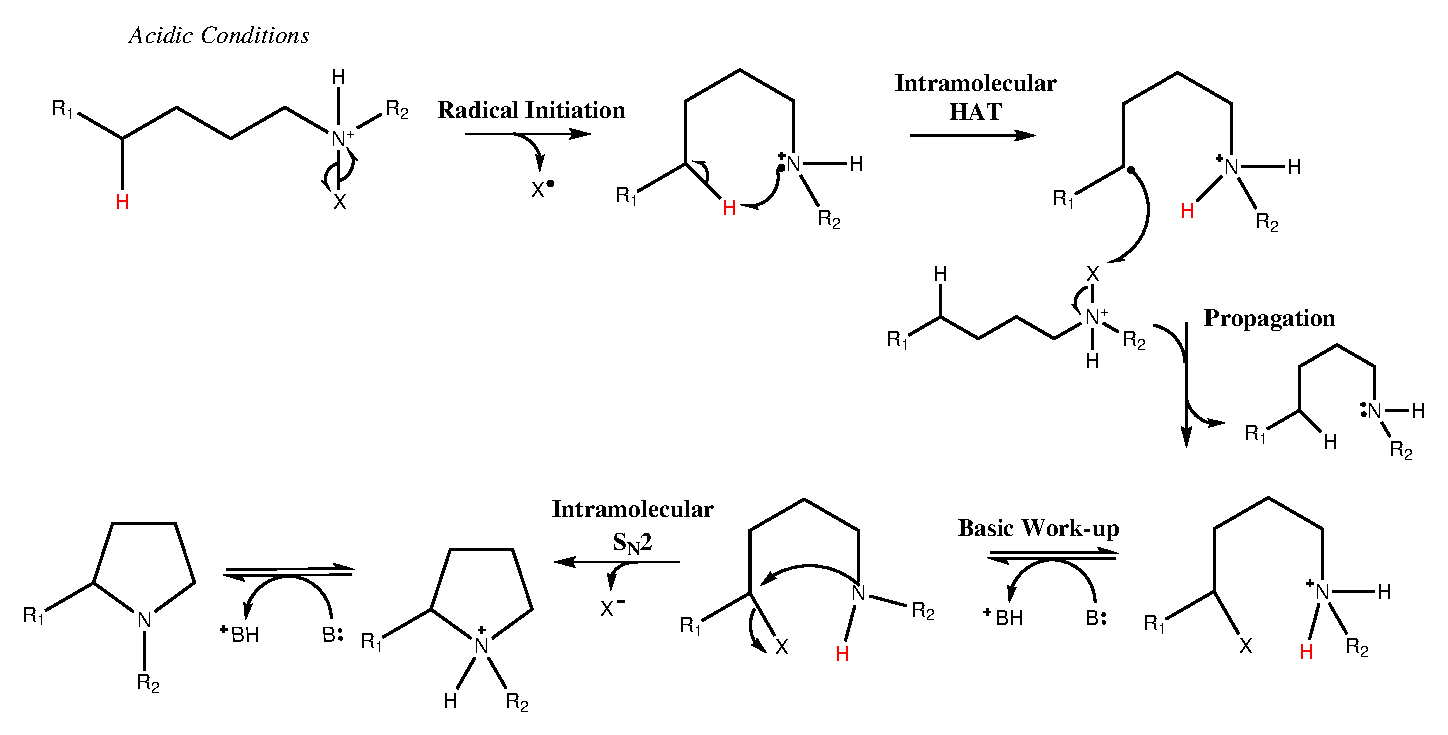
\includegraphics[width=\textwidth]{figures/hofmann.eps}
  \caption[Reaction mechanism of the Hofmann-L{\"o}fler-Freytag reaction]{
    Reaction mechanism of the Hofmann-L{\"o}fler-Freytag reaction. The reaction
    proceeds under acidic conditions so that the amine is protonated. Step one
    is radical initiation, typically through radiation or a radical initiator,
    step two is the intramolecular HAT reaction, step three is the propagation
    of the radical activating addition amines and abstracting a halide, step
    four begins the basic work up with deprotonation of the amine, followed by
    $S_N2$ attack of the $\delta$ position with a halide, and finally the second
    deprotonation of the amine centre.}
\label{fig:hofmann}
  \end{center}
\end{scheme}

Since the early days of Hofmann, a great deal of work has been done, and new
methods for C-H functionalisation have been achieved. The most commonly used
technique is the hydroxylation of C-H bonds, which then serve as a synthetic
handle. Transition metal chemistry is now typically employed to achieve C-H bond
functionalisation. This often involves highly reactive metal-oxo intermediates
responsible for triggering C-H bond cleavage, with an inorganic HAT reaction
being an essential part of the mechanism.\cite{Groves1976} Reactions of this
nature are subject to low selectivity and complex product mixtures due to the
similarly thermodynamics and kinetics of hydroxylation and dehydrogenation
pathways.\cite{Balcells2016} A similar mechanism is found in metalloenzymes,
which prompted important work investigating the selectivity and tunability of
these reactions, with considerable success. This work along several works of
others,\cite{Miller2016} are exemplary cases where a detailed understanding of
the HAT reaction mechanism can lead to significant contributions to chemistry.

\newpage

\section{Physico-chemical determinants of formal hydrogen transfer reactions}

Given the importance of HAT reactions in biology and chemistry, a thorough
understanding of these reactions is clearly important. In order to fully
understand HAT reactions, we much understand the factors which influence these
reactions.

\subsection{Understanding chemical reactions}

The potential energy surface (PES) for any chemical reaction is a complex
hypersurface that depends on many variables. Typically this problem can be
simplified by examining only the relevant geometry changes. Often the two most
important coordinates can be isolated, giving a 3-dimensional potential energy
surface. Furthermore, in chemistry we simplify this problem to 2-dimensions,
such that the so-called intrinsic reaction coordinate, or the lowest energy
cross section of a higher dimension PES.\@ This yields a reaction coordinate
diagram, as is illustrated below in~\ref{fig:pes}.

\begin{figure}[htb]
  \centering
  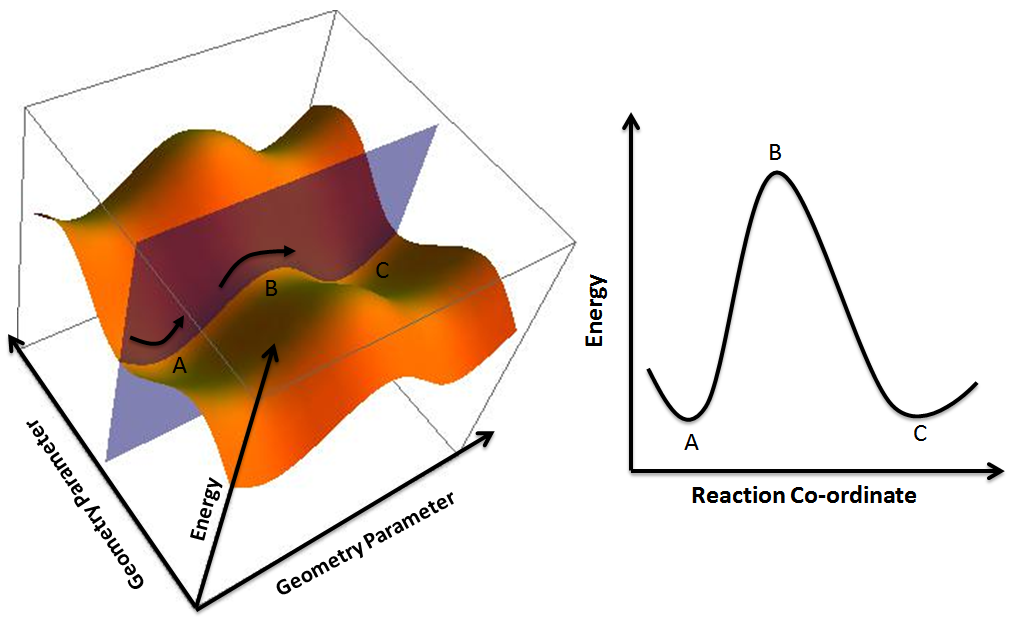
\includegraphics[width=0.9\textwidth]{figures/pes}
  \caption{Placeholder PES from Wikipedia}
\label{fig:pes}
\end{figure}

\noindent In a typical reaction coordinate diagram, the reactants begin to
interact and form a pre-reaction complex (A). Given sufficient energy, the
reaction will proceed over the top of the energy barrier through a transition
state (TS) complex (B). After the chemical transformation is completed, a
post-reaction complex (C) is formed until the products are able to separate.

In quantum chemistry, we are generally not concerned with the dynamics of a
chemical reaction, but rather the thermodynamic and kinetic properties of a
reaction. This is achieved through the investigation of stationary states
(reactants, pre-reaction complex, TS complex, post-reaction complex, and
products) along the reaction coordinate. Thermodynamic analysis of a reaction
requires the understanding of the stability of the products relative to the
reactants, measured by change in Gibbs free energy $\Delta G$, while kinetic
analysis requires the understanding of the stability of the TS complex relative
to the reactants measured by the Gibbs free energy
barrier $\Delta G^{\ddagger}$.\jnote{Need to modify figure to include energy}

To fully understand HAT reactions, one must analyse the factors which influence
the thermodynamics and kinetics of these reactions. Thermodynamically this is
relatively simple; the most important factor to consider is relative bond
strengths. Typically, a reaction will be exergonic if the bond being formed is
stronger than the bond being broken. Entropic changes ($\Delta S$) in HAT
reactions are in all but the most unusual cases, negligible
($\Delta S \approx 0$).\cite{Mader2007} Kinetic analysis can be considerably
more complicated, as there are numerous factors which can stabilise or
destabilise the reactants or TS complex. The important factors include solvent
interactions, non-covalent interactions, bond strengths, and stereo-electronic
interactions, each of which is described below.

\subsection{Factors influencing the kinetics of HAT reactions}

\subsubsection{Solvent interactions}

Kinetic solvent effects (KSEs) describe the effect on a reaction from solvent
interactions. Solvent has the ability to stabilise or destabilise the TS complex
of a HAT reaction. Since the earliest studies describing KSEs in
1964,\cite{Howard1964} a great deal of literature exists describing KSEs,
especially for HAT reactions involving phenols.\cite{note2} Hydrogen bond (HB)
formation between phenols and HB accepting solvents is attributed to the
observation that increasing solvent polarity decreases the rate constants for
HAT reactions ($k_H$). Unlike phenols, our amide models possess an HB accepting
moiety, and thus interact strongly with HB donating solvents. Experimental work
from our colleagues in Rome has demonstrated that for C-H bond HAT from
substrates with HB accepting capabilities, $k_H$ decreases with solvent HB
donating ability. Evidence for this is summarized in~\ref{tab:kse}: for HAT
reactions of \cumo with $N,N$-dimethylformamide (DMF), tetrahydrofuran (THF),
and triethylamine (TEA), as the polarity and HB donating ability of the solvent
increases, the rate constant $k_H$, decreases.


\begin{table}[htb]
{\footnotesize
\centering
  \begin{tabular}{l r r r}
    Solvent & $N,N$-dimethylformamide$^a$ & Tetrahydrofuran$^b$ & Triethylamine$^c$ \\
\toprule
\toprule
    isooctane & (7.7 $\pm$ 0.1) $\times 10^6$ & (1.21 $\pm$ 0.02) $\times 10^7$ & \rule{0pt}{3ex} (2.9 $\pm$ 0.1) $\times 10^8$  \\
    benzene & (3.1 $\pm$ 0.1) $\times 10^6$ & (7.2 $\pm$ 0.7) $\times 10^6$ & (2.8 $\pm$ 0.1) $\times 10^8$ \\
    MeCN & (1.24 $\pm$ 0.02) $\times 10^6$ & (5.8 $\pm$ 0.2) $\times 10^6$ & (2.0 $\pm$ 0.1) $\times 10^8$ \\
    $t$-BuOH & (1.38 $\pm$ 0.03) $\times 10^6$ & (5.8 $\pm$ 0.2) $\times 10^6$ & (1.61 $\pm$ 0.03) $\times 10^8$ \\
    MeOH & (9.8 $\pm$ 0.2) $\times 10^5$ & (4.9 $\pm$ 0.2) $\times 10^6$ & (3.8 $\pm$ 0.1) $\times 10^6$ \\
    TFE & $<$ 1 $\times 10^4$ & (2.7 $\pm$ 0.1) $\times 10^6$ & \\
  \end{tabular}
  \caption[Summary of second-order rate constants for HAT from C-H bonds for
  hydrogen bond accepting substrates from the cumyloxyl radical.]{Second-order
    rate constants ($k_H$, \Ms) for HAT from C-H bonds of hydrogen bond
    accepting substrates to the cumyloxyl radical measured in different
    solvents at 25 $^{\circ}$C. $^a$Reference
    \citenum{Salamone2015}. $^b$Reference \citenum{Salamone2014Syn} and
    \citenum{Bietti2011}. $^c$Reference \citenum{Bietti2010}.}
2\label{tab:kse}
}
\end{table}


The KSEs observed in~\ref{tab:kse} can been explained on the basis of
hyperconjugation, the donation of electron density from neighbouring orbitals
into C-H $\sigma^*$ antibonding orbitals. Hyperconjugation has a net stabilising
effect, however it decreases the strength of C-H bonds by accepting electron
density into a C-H $\sigma^*$ orbital. For the species listed in~\ref{tab:kse},
abstraction occurs primarily from C-H bonds adjacent to a heteroatom or $\pi$
system. Hyperconjugative overlap between the heteroatom and C-H $\sigma^*$
antibonding orbitals in these species is decreased by the formation of a
hydrogen bond with solvent, effectively increasing the strength of the C-H bond
and thus destabilising the TS complex and increasing $\Delta G^{\ddagger}$. This
is the key kinetic effect of solvation in the our model systems.


\subsubsection{Non-covalent interactions}

Non-covalent interactions (NCIs; eg.\ van der Waals interactions, hydrogen
bonding, etc.)  play a central role in all chemistry. It has already been
demonstrated that HB formation between substrates and solvents plays an
important role, however oxygen centres can also hydrogen bond with substrates as
both acceptors and donors.\cite{Johnson2009a} These hydrogen bonding
interactions, in addition to the other non-covalent interactions between the
radical and substrate lead to the formation of a pre-reaction complex. No
literature currently exists which discusses how the strengths of these
interactions impacts the kinetics of a reaction, however these effects cannot be
ignored. Chapter~\ref{ch:arrhenius} of this thesis shall deal with this specifically.

Non-covalent interactions are known to be important in the stabilisation of TS
complexes in HAT reactions.\cite{DiLabio2005,DiLabio2007} Although the effects
of NCI stabilisation are difficult to quantify, the concept of TS complex
stabilisation is being recognised in applications such as enzyme
catalysis\cite{Uyeda2011} and synthetic catalysis.\cite{Bakr2016}

It has been demonstrated that the formation of pre-reaction complexes can in
fact be the rate-limiting step of a
reaction.\cite{Salamone2011,Salamone2011a,Salamone2013a} Combined experimental
and computational examinations of HAT reactions between the cumyloxyl (\cumo) or
benzyloxyl (\bno) radicals with tertiary alkylamines and alkylamides
demonstrated that the relatively acidic $\alpha$-C-H of \bno is capable of
forming hydrogen bonds with enthalpies ($\Delta H$) of 4.0 \kcalmol for
alkylamines to 8.5 \kcalmol in alkylamides. The comparison of $k_H$ for these
HAT reactions between \cumo and \bno ($k_H^{BnO}/k_H^{CumO}$) demonstrates large
rate enhancements, ranging from 2.8 for the very sterically hindered
triisobutylamine, to 1094 for 1,4-diazabicyclo[2.2.2]octane. In this case, NCIs
control the kinetics of the reaction not through stabilisation, but rather
through changing the rate-determining step.


\subsubsection{Bond strengths and the Bell-Evans-Polanyi Principle}

It has long been the interest of chemists to understand chemical reactions from
both a thermodynamic and kinetic standpoint. The measurement and comparison of
bond strengths, that is bond dissociation enthalpies (BDEs), is central to the
understanding of reactivity with respect to thermodynamics. There exists a
tremendous amount of literature in which BDEs are linked to chemical reactivity,
especially for HAT
reactions.\cite{Kochi1973,Tedder1982,Wijtmans2003,Pratt2004,Mayer2004}

Often, BDEs are used in linear free energy relationships (LFERs) to relate
chemical reactivity to bond strength. One such example\cite{Pratt2004} is the
application of BDEs to the Hammett equation\cite{Anslyn2006}, which can be used
to study substituent effects from thermodynamic (Equation
\ref{eq:hammettthermo}) or kinetic analysis (Equation~\ref{eq:hammettkin}).

\begin{align}
 \log\frac{K_X}{K_H} &= \rho \sigma_X \label{eq:hammettthermo} \\
 \log\frac{k_X}{k_H} &= \rho \sigma_X \label{eq:hammettkin}
\end{align}

\noindent In the above equations, $K$ is an equilibrium constant and $k$ is a
rate constant for either a reference reaction with a hydrogen substituent $H$ or
a given substituent $X$. The substituent parameters $\sigma_X$, have been
measured for various different reference reactions, although the original
parameters were measured for the acidity of benzoic acid.\cite{Hammett1937}
~Plots of $\log(K_X/K_H)$ or $\log(k_X/k_H)$ against $\sigma_x$ have been used
to determine $\rho$, the sensitivity constant. Originally $\rho$ was used to
determine whether a reaction was more sensitive ($\rho > 1$), less sensitive
($\rho < 1$), or equally sensitive to substituents than benzoic acid, with
negative charges being produced. If $\rho$ is negative then positive charge is
said to be formed as a result of substituents.

In the context of BDEs, \citet{Pratt2004} examined a series of substituents (Y)
on toluenes, anilines, and phenols (4-\ch{YC6H4-ZX}), and showed that the Z-X
BDEs can be correlated to the electrophilic substituent constants,
$\sigma_p^+($Y). This was surprising because it demonstrated that homolytic
properties correlated with properties derived from the heterolytic $S_N1$
solvolyses of para-substituted cumyl chlorides.\cite{Brown1958} Specifically,
this showed that since $\sigma_p^+($Y) describes the relative ability of Y to
stabilise a positive charge, the ability to stabilise strong electron
withdrawing (EW) moieties can be well described in general by these
parameters. This means that BDEs for toluenes and anilines are well correlated
to $\sigma_p^+($Y), since \ch{O^.} and \ch{NH^.} can be described like positive
charges (strong EW groups). Toluenes, which have resulting radicals (\ch{CH2^.})
which are neither electron withdrawing nor donating, are poorly correlated with
$\sigma_p^+($Y).

Another interesting LFER, which is utilised in Chapter~\ref{ch:bde}, is the
Bell-Evans-Polanyi (BEP) Principle,\cite{Bell1936,Evans1938} which states that
the difference in activation energy ($E_a$) for two related reactions (within
the same family), is proportional to the differences in reaction enthalpy
($\Delta H$):

\begin{align}
  E_a = E_0 + \alpha \Delta H
  \label{eq:bep}
\end{align}

\noindent This relationship has been more generally used to compare larger
families of reactions. The remaining terms in Equation~\ref{eq:bep} are $E_0$,
the activation energy of a reference reaction, and $\alpha$ is a constant which
characterises the position of the TS along the reaction coordinate. This can be
rationalised by considering a series of reactions with similar energy profiles:
if the reaction becomes more exothermic, the barrier height will decrease (the
opposite is also true for endothermic reactions), as illustrated in
\ref{fig:bep}.

\begin{figure}[htb]
  \centering
  
\includegraphics[width=0.7\textwidth]{figures/bep}
  \caption{Energy profiles for a series of related exothermic reactions
    illustrating the Bell-Evans-Polanyi Principle.}
\label{fig:bep}
\end{figure}

If the BEP relationship holds for a series of related HAT reactions, then BDEs
should correlate with the activation energy, where increased bond strengths
would represent a destabilisation in the TS complex. In practice, plots of BDEs
against the logarithm of rate constant are used. An interesting example of this
is the work of \citet{Pratt2003}, in which the free radical oxidation of
unsaturated lipids is examined. They achieve this through the correlation of
theoretically determined C-H and \ch{C-OO^.} bond strengths with experimentally
measured HAT rate constants and \ch{O2} addition rate constants,
respectively. BEP plots (BDE vs. $\log k$) for a large range of polyunsaturated
fatty acid models show good correlation for both the C-H bonds and \ch{C-OO^.}
bonds examined. This demonstrates that BDEs have a direct impact on the reaction
barrier height, giving validation to the BEP Principle.

Although chemists often consider the importance of BDE in thermodynamic
analysis, bond strengths are an important consideration in kinetic analysis as
well. As such, the altering of bond strengths can be an important factor in
related HAT reactions. The generallity of application of the BEP Principle is
discussed in Chapter~\ref{ch:bde}.

\subsubsection{Stereo-Electronic interactions}

The effects of sterics and electronics have been shown to play an important role
in HAT reactions. Generally, these effects are described as two seperate
phenomena: polar effects and steric effects.

The species involved in HAT reactions are often neutral radicals, thus the
influence of charge transfer in the TS complex can have important
implications. Consider the TS of a generic HAT reaction in~\ref{fig:hatts},
there are four obvious resonance forms. For a series of related reactions, $E_a$
would be expected to decrease as the contribution of dipolar ion resonance forms
increases.\cite{Roberts1999} Oxygen centred radicals are electrophilic in
nature, thus the importance of the third resonance structure becomes
important. HAT is favoured from C-H bonds which are electron rich, or
nucleophilic.\cite{Salamone2015Rev}

\begin{scheme}[htb]
  {\huge\ch{[X-H-Y]}$^\ddagger$} \\
  \vspace{0.5cm}
  {\large
  \ch{[X^.H-Y]}$^\ddagger$ \ch{<-> [X-H Y^.]}$^\ddagger$ \ch{<->
    [X:^-H^.Y^+]}$^\ddagger$ \ch{<-> [X^+H^.Y:^-]}$^\ddagger$}
  \caption{A generic HAT transition state structures and possible resonance forms.}
\label{fig:hatts}
\end{scheme}

An example of this effect is from the work of our colleagues in
Rome,\cite{Bietti2011,Salamone2012} in which rate constants ($k_H$, normalised
for the number of abstractable hydrogens) for cyclohexane and acetone to the
cumyloxyl radical (\cumo) were measured and compared to theoretically determined
C-H BDEs. Cyclohexane has a C-H BDE = 99.5 \kcalmol and $k_H$ = $9.2\times10^4$
\Ms, while acetone has C-H BDE of 96.0 \kcalmol and $k_H$ = $ < 2\times10^3$
\Ms.\ \ As a result of polar effects, although cyclohexane has a greater bond
strength, it is at least an order of magnitude more reactive in HAT than
acetone.

The effects of steric bulk also play an important role in HAT, and have been
studied extensively by our colleagues in Rome, as well as by
others.\cite{Finn2004,Salamone2011,Pischel2001,Griller1981,Bietti2011,
  Salamone2012,Malatesta1982,Salamone2014} Although a C-H bond may be weaker
than others on a given substrate, if it is not accessible due to steric
constraints, abstraction will not occur at this site. Otherwise, additional
steric bulk can lead to significant reductions in reactivity, through
destabilisation of the TS complex. For example, in reactions of tertiary
acetamides with \cumo,\cite{Salamone2014} where abstraction occurs mainly from
C-H bonds $\alpha$ to the nitrogen atom, a two fold decrease in normalised rate
constant is observed in going from $N,N$-dimethylacetamide to
$N,N$-diisobutylacetamide ($k_H$ = $2.0 \times 10^5$ and $7.8 \times 10^4$ \Ms,
respectively).

\subsection{Mechanistic details of hydrogen transfer reactions}

For a simple HAT reaction, as shown in~\ref{fig:hat}, there exists several
possible mechanisms by which this transformation can occur. The two most common
concerted mechanisms are direct HAT\cite{note1}~and proton-coupled electron
transfer (PCET). At the basic level, direct HAT involves the transfer of an
electron and proton through the same set of acceptor/donor orbitals, while PCET
involves the transfer of an electron and proton through different sets of
orbitals. In practise, this distinction is poorly described and this topic is
still in active discussion in the
literature.\cite{Cukier1998,Mayer2002,Stubbe2003,Mayer2004,DiLabio2007,Huynh2007,Hammes-Schiffer2008,Mayer2010,Weinberg2012,Hammes-Schiffer2015,Munoz-Rugeles2017}
Primarily, the distinction between the two processes is unclear because the two
processes cannot be entirely separated physically.\cite{DiLabio2007}

\begin{scheme}[htb]
  \begin{center}
    
\includegraphics[width=0.75\textwidth]{figures/FHT.eps}
  \caption{A generic formal hydrogen transfer reaction.}
\label{fig:hat}
  \end{center}
\end{scheme}

The quintessential example when comparing direct HAT to PCET is the
self-exchange reactions of benzyl/toluene and phenoxyl/phenol shown in
\ref{fig:self1}, as described by \citet{Mayer2002}.

% \begin{align}
% \ch{ % C6H5CH2-H + C6H5CH2^. &-> C6H5CH2^. + C6H5CH2-H} \label{eq:self1} \\
% \ch{ % C6H5O-H + C6H5O^. &-> C6H5O^. +C6H5O-H} \label{eq:self2}
% \end{align}


\begin{scheme}[htb]
\begin{center}
  \textbf{A. }\\
    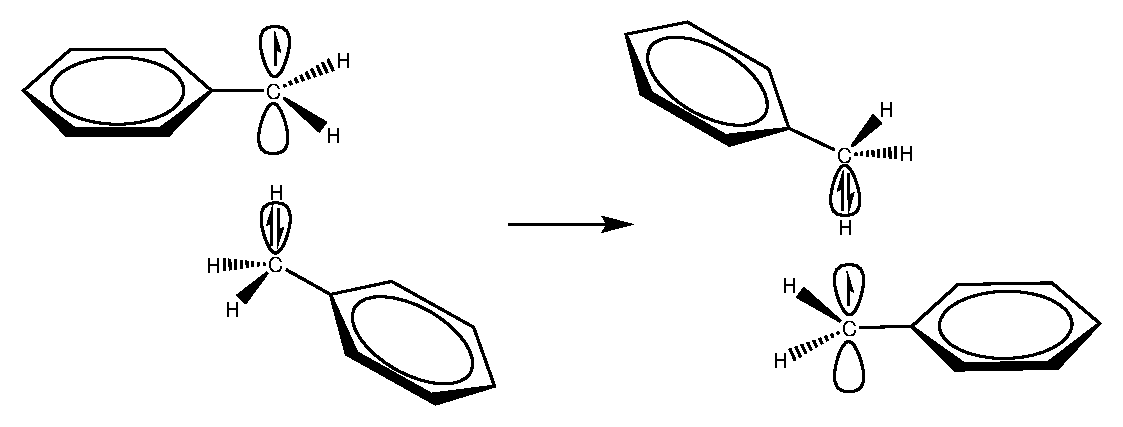
\includegraphics[width=0.75\textwidth]{figures/PhCH3-PhCH2.eps}\\
  \textbf{B. }\\
    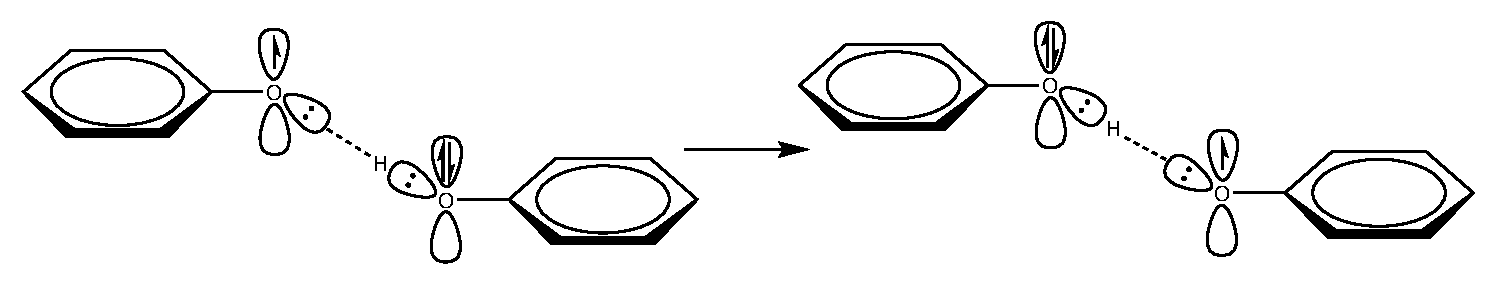
\includegraphics[width=0.95\textwidth]{figures/PhOH-PhO.eps}\\
    \caption{Self-exchange reactions of the \textbf{A.} benzyl/toluene couple
      through direct HAT \textbf{B.} phenoxyl/phenol couple through PCET.}
\label{fig:self1}
\end{center}
\end{scheme}

In this work, the transition state structures, obtained through theoretical studies, were reported. The proposed structures have $C_{2h}$ and $C_2$ symmetry for~\ref{fig:self1} A and B, respectively, oriented so that the aromatic rings are trans relative to one another. In this geometry, the benzyl/toluene pair undergoes direct HAT, with the $2p-\pi$ orbital of the benzylic carbon radical oriented at the benzylic hydrogen on toluene and little delocalisation of the radical into the $\pi$-system. Additionally, the singly occupied molecular orbital (SOMO) is of $\sigma$ symmetry. The calculated enthalpic barrier ($\Delta H^{\ddagger}$) is 17.7 \kcalmol. For the phenoxyl/phenol pair, a fairly strongly hydrogen bonded pre-reaction complex is first formed (-8.1 \kcalmol, relative to reactants). The TS structure is such that the phenoxyl radical occupies a $2p$ orbital, and is allowed to overlap with the $2p$ lone pair of the phenol moiety and the aromatic $\pi$ systems. This demonstrates that the SOMO is of $\pi$ symmetry and highly delocalised, and that HAT occurs through a PCET mechanism. The reaction has a barrier height $\Delta H^{\ddagger}$ = 5.0 \kcalmol relative to the hydrogen bonded complex, so that the barrier is 3.1 \kcalmol below the separated reactants.

The work by \citet{Mayer2002} suggests that hydrogen bonding is a necessary, but not sufficient condition for PCET to occur. This then implies that PCET is not possible between molecules which do not possess hydrogen bonding moieties, such as carbon atoms. Work by other authors has shown this to be untrue.\cite{Hatcher2007,DiLabio2007} In particular, \citet{DiLabio2007} demonstrated that this neglected the important contributions of $\pi-\pi$ interactions and lone pair-$\pi$ interactions. Additional calculations revealed there exists a TS structure for the benzyl/toluene couple which is 3.7 \kcalmol lower in energy than previously reported. This structure has $C_2$ symmetry with the aromatic rings oriented $34^\circ$ relative to one another, allowing for optimal $\pi$-stacking, and thus $\pi-\pi$ overlap opens up an electronic channel for PCET to occur. They also suggest that the phenol/phenoxyl couple likely prefers a $\pi$-stacked TS structure, and compare this to a structural analogue, a naturally occuring tyrosyl/tyrosine couple. Additional work by \citet{Munoz-Rugeles2017} confirmed the existance of a $\pi$-stacked TS structure for the phenol/phenoxyl couple. They used an approach which utilises natural population analysis along the intrinsic reaction coordinate, and demonstrated that both the benzyl/toluene couple and phenoxyl/phenol couple favour a $\pi$-stacked TS structure and undergo HAT through a PCET mechanism. Interestingly, they also showed that reaction barrier heights for the PCET mechanism are systematically lower than those for direct HAT.

As there is not an obvious way to explore the differences in mechanism experimentally, computational examination of formal HAT reactions enables analysis of the mechanism of these reactions. Using a variety of tools, a general distinction between a HAT mechanism and PCET mechanism can be achieved, however, as stated previously, these mechanisms are not mutually exclusive. Regardless, important insight can be gained from understanding the electronic behaviour of these reactions.


\subsection{The effects of metal cations on HAT reactions}

Solvent interactions in HAT reactions can be described as Lewis acid/base
interactions. In biological systems, the most common solvent is water, which can
act as both a Lewis acid and base, due to its self-ionising equilibrium. Other
important Lewis acids in biology are the non-redox active alkali and alkaline
earth metal cations that are present ubiquitously throughout biological
systems. Metal ions such as sodium, magnesium, potassium, and calcium are
essential to biological function.\cite{Karp2013} \jnote{Include something about
  number of ions per protein and/or biological concentrations}

Given the Lewis acid/base nature of these non-redox active metals, we were
driven to explore the effects upon HAT reactions. Experimental investigation of
these effects has been underway by the Bietti group in Rome. The effects of
non-redox active metal cations on HAT from C-H bonds of cyclohexadiene (CHD),
tetrahydrofuran (THF), and tertiary alkylamines to \cumo were
examined.\cite{Salamone2013} This work is summarized in
\ref{tab:expcations}. Additional experiments examining the same reactions of
$N,N$-dimethylacetamide (DMA) and $N,N$-dimethylformamide
(DMF)\cite{Salamone2015}, as well as for various other
acetylamides\cite{Salamone2016} have been performed, and provides the
experimental background for this thesis.

\begin{table}[htb]
{\footnotesize
  \centering
  \begin{tabular}{c l r}
 Substrate & Conditions & $k_H($\Ms) \\
 \toprule
 \toprule
CHD & \rule{0pt}{3ex}            & (6.65 $\pm$ 0.02) $\times 10^7$ \\
        & \ch{LiClO4} 1.0 M       & (7.49 $\pm$ 0.04) $\times 10^7$ \\
        & \ch{Mg(ClO4)2} 1.0 M & (7.0 $\pm$ 0.1) $\times 10^7$ \\
\midrule
THF  &                                    & (5.7 $\pm$ 0.1) $\times 10^6$ \\
        & \ch{LiClO4} 1.0 M       & (2.87 $\pm$ 0.04) $\times 10^6$ \\
        & LiOTf 1.0 M                & (2.8 $\pm$ 0.2) $\times 10^6$ \\
        & \ch{Mg(ClO4)2} 1.0 M & (1.8$\pm$ 0.1) $\times 10^6$ \\
\midrule
TEA  &                      & (2.0 $\pm$ 0.1) $\times 10^8$ \\
        & \ch{LiClO4} 1.0 M           & (9.37 $\pm$ 0.01) $\times 10^7$ \\
        & \ch{Mg(ClO4)2} 0.005 M & $<$ 1 $\times 10^{6*}$ \\
\midrule
PMP  &                                       & (1.70 $\pm$ 0.02) $\times 10^8$ \\
        & \ch{LiClO4} 1.0 M           & (9.0 $\pm$ 0.3) $\times 10^ 7$ \\
        & \ch{Mg(ClO4)2} 0.005 M & $<$ 1$\times 10^{6*}$
  \end{tabular}
  \caption[Summary of experimental rate constants of HAT with \cumo for
  cyclohexadiene (CHD), tetrahyrofuran (THF), triethylamine (TEA), and
  1,2,2,6,6-pentamethylpiperidine (PMP), including the effect of non-redox
  active metal cations.]{Summary of experimental rate constants of HAT with
  \cumo for cyclohexadiene (CHD), tetrahyrofuran (THF), triethylamine (TEA), and
  1,2,2,6,6-pentamethylpiperidine (PMP), including the effect of non-redox
  active metal cations. Rate constants were determined by LFP in 25 $^{\circ}$C
  MeCN.\@ $^*$Rate constants are approximate as the effects of even small
  additions of metal cations cause rate outside the range of laser flash
  photolysis experiments.}
\label{tab:expcations}
}
\end{table}

In general, metal cation interactions lead to deactivation of C-H bonds and
experimental rate constants decrease as a result. An explaination for this is
the same as for KSEs, where Lewis acid binding causes a decrease in $\alpha$-C-H
bond $\sigma^*$ population, thus increasing the effective C-H bond strength and
decreasing $k_H$. For cyclohexadiene, a marginal increase in $k_H$ was observed
with additions of 1.0 M \ch{LiClO4} and \ch{Mg(ClO4)2}, which was explained on
the basis of interactions of the metals with \cumo. This demonstrates that metal
cations have a limited ability to influence HAT reactions of \cumo with alkene
based substrates. For THF, $k_H$ is 2.0 and 3.2 times lower with the addition of
1.0 M \ch{LiClO4} and \ch{Mg(ClO4)2}, respectively. \ch{LiClO4} has a roughly
2-fold decreasing effect on $k_H$ for alkylamines, whereas \ch{Mg(ClO4)2} has a
significantly greater effect, decreasing $k_H$ by more than two orders of
magnitude, an effect that has been attributed to the compact charge density of
\ch{Mg^{2+}}. As a whole, these results suggest that metal ions interact more
strongly with substrates than \cumo, thus C-H bond deactivation is observed due
to Lewis acid/base effect. The Lewis acidity of the metal appears to have an
important role, since \ch{Mg(ClO4)2} $>$ \ch{LiClO4} in regards to Lewis acidity
and effect on $k_H$. The Lewis basicity of the substrate is also clearly
important. Alkylamines undergo a larger decrease in $k_H$, relative to THF, as
they are stronger Lewis bases. Computational studies have validated these
results, demonstrating that binding of \ch{Mg(ClO4)2} leads to a 5.1 \kcalmol
decrease in the $\alpha$-C-H BDE in TEA and that $k_H$ decreases by
$>4$ orders of magnitude.\cite{Nova2014}

Simple amides such as DMF and DMA are often used as simple peptide
models.\cite{Salamone2015a} As such the deactivation of C-H bonds in amides, as
indicated by the observed decreases in $k_H$, leads to the central hypothesis of
this thesis: \emph{non-redox active metals cations can serve as chemoprotective
  agents for biomolecules}. Experimental evidence for this is demonstrated in
\ref{fig:expdmadmf}. For \ch{LiClO4} added to DMF and DMA, total inhibition of
HAT occurs up to 2 and 1 molar equivalents, respectively. Inhibition of HAT
occurs for 2 and 4 molar equivalents, respectively, followed by total
non-inhibition. A much weaker effect is observed with \ch{NaClO4}, while a
similar strong deactivating effect is observed for \ch{Ca(ClO4)2}. The addition
of \ch{Mg(ClO4)2} gives weak deactivation for the first two molar equivalents of
both DMF and DMA, with strong activation for an additional two equivalents. This
unusual behaviour is as of yet, unexplained. Additional discussion of
experimental results shall be reserved for Chapter~\ref{ch:hat}.

\begin{figure}[htb]
  \centering
  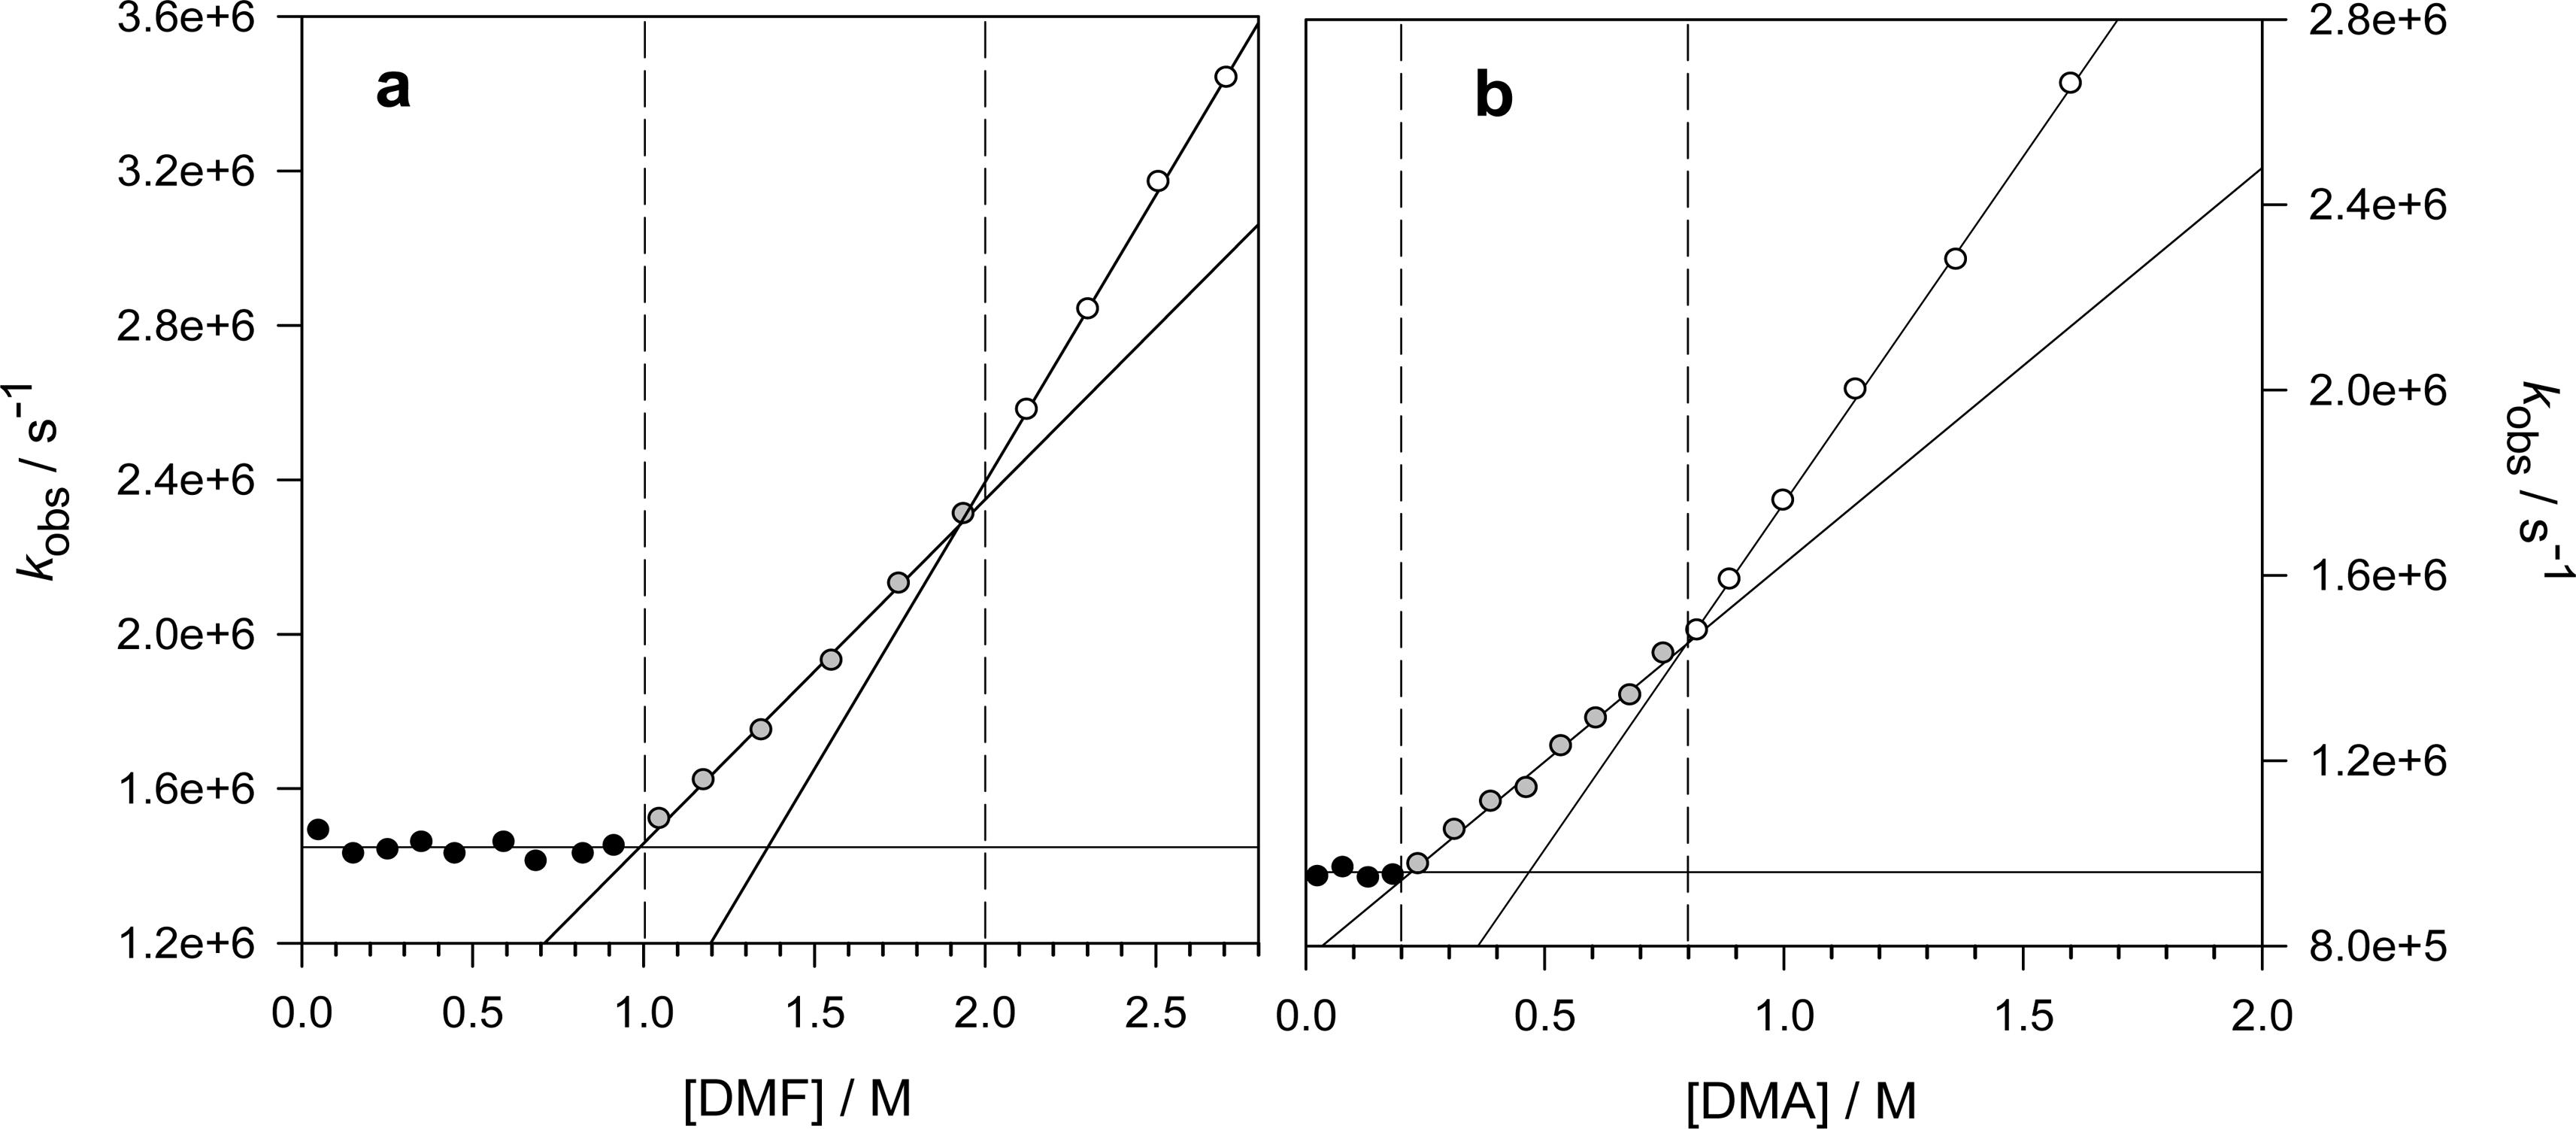
\includegraphics[width=0.9\textwidth]{figures/exptdmadmf}
  \caption[Plots of observed rate constants against concentration of substrate for HAT
  reactions with cumyloxyl radical.]{Plots of observed rate constants against
    concentation of substrate for HAT reactions with cumyloxyl radical: \textbf{a}
    Substrate = DMF, measured by LFP at 25$^{\circ}$C in solutions of MeCN
    containing 1.0 M dicumyl peroxide and 0.5 M \ch{LiClO4}. Complete inhibition
    of HAT is observed at 0--1.0 M, while linear regression for the 1.0--2.0
    M regions gives $k_{H1}$ = 8.91 $\times 10^5$ \Ms, and $k_{H2}$ = 1.49
    $\time 10^6$ \Ms in the 2.0--2.7 M region. \textbf{b} Substrate = DMA,
    measured by LFP at 25 $^{\circ}$C in solutions of MeCN containing 1.0 M
    dicumyl peroxide and 0.2 M \ch{LiClO4}. Complete inhibition of HAT is
    observed at 0--0.2 M, while linear regression in the 0.2--0.8 M
    region gives $k_{H1}$=8.54 $\times 10^5$ \Ms and $k_{H2}$ = 1.49
    $\times 10^6$ \Ms in the 0.8--1.6 M region. Figure taken from Reference
    \citenum{Salamone2015}.}
\label{fig:expdmadmf}
\end{figure}


\newpage
% \section{Research hypotheses and objectives}
% \label{sec:hypotheses}

% Hydrogen atom transfer reactions represent a simple, yet important chemical
% transformation that is relevant to many fields of study. It is therefore
% important that these reactions be as well-defined and understood as
% possible. The ideal tool for this is the combined experimental and computational
% study of model systems. The understanding gained from these systems should be
% applicable to other chemical species, therefore giving important insight into
% the biological and chemical processes which are studied now and in the future. The
% following two chapters shall serve as the theoretical background (Chapter
% \ref{ch:theory}) for the theoretical procedures employed (Chapter
% \ref{ch:methods}) to investigate several key hypotheses: There exists a
% relationship between the non-covalent binding and Arrhenius pre-factors (Chapter
% \ref{ch:arrhenius}); the Bell-Evans-Polanyi Principle may be applicable for
% aliphatic C-H bonds as a whole, and may (or probably doesn't now?) apply to all
% other alkyl C-H bonds (Chapter \ref{ch:bde}); and non-redox active metal
% cations exhibit a chemoprotective effect against abstraction by oxygen centered
% radicals in biologically and chemically relevant substrates (Chapter
% \ref{ch:hat}).

% These hypotheses were explored through the following objectives:

% \textbf{Chapter 4}
% \begin{itemize}
% \item To determine the global minimum structures of hydrogen-bonded pre-reaction
%   complexes for near thermoneutral HAT reaction which have experimental results.

% \item To determine accurate binding energies that can be used to correlate with
%   experimentally determined Arrhenius pre-factors.

% \item To obtain transition state structures that can be used to test or validate
%   computational methods for the determination of kinetic properties of HAT
%   reactions.
% \end{itemize}

% \textbf{Chapter 5}
% \begin{itemize}
% \item To obtain highly-accurate bond dissociation enthalpies for C-H bonds for
%   which experimental rate constants have been determined.

% \item To prepare and analyse Bell-Evans-Polanyi plots of the obtained data and
%   determine if there exists two linear relationships for allylic and alkyl C-H
%   bonds.
% \end{itemize}

% \textbf{Chapter 6}
% \begin{itemize}
% \item To benchmark density-functional theory methods for the interactions of
%   non-redox active metal cations with organic substrates and molecules.

% \item To evaluate the effects of non-redox active metal binding on HAT reaction
%   barrier heights involving simple protein models (amides), as well as various
%   common organic solvents.
% \end{itemize}

%%% Local Variables:
%%% mode: latex
%%% TeX-master: "diss"
%%% End:
